\begin{figure}[t]
\centering
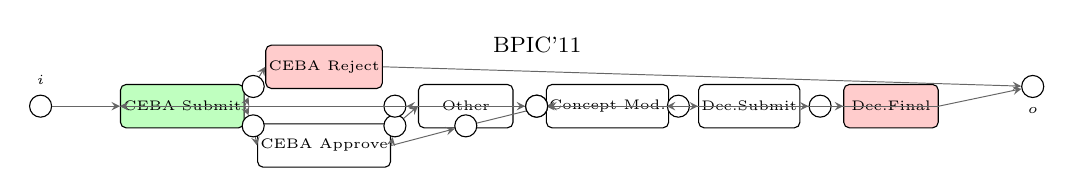
\begin{tikzpicture}[
    transition/.style={rectangle, rounded corners=2pt, draw=black, fill=white,
        minimum width=1.2cm, minimum height=0.55cm, align=center, font=\tiny,
        inner sep=1pt, line width=0.4pt},
    place/.style={circle, draw=black, fill=white,
        minimum size=0.28cm, inner sep=0pt, line width=0.4pt},
    post/.style={line width=0.35pt, draw=black!60},
]
\colorlet{startcolor}{green!25}
\colorlet{endcolor}{red!20}
\colorlet{transitioncolor}{white}
  % Petri net for BPIC'11
  \node[transition, fill=startcolor] (t_bpic2011_0) at (0.0, 0.0) {\tiny CEBA Submit};
  \node[transition, fill=transitioncolor] (t_bpic2011_1) at (1.8, -0.5) {\tiny CEBA Approve};
  \node[transition, fill=endcolor] (t_bpic2011_2) at (1.8, 0.5) {\tiny CEBA Reject};
  \node[transition, fill=transitioncolor] (t_bpic2011_3) at (5.4, 0.0) {\tiny Concept Mod.};
  \node[transition, fill=transitioncolor] (t_bpic2011_4) at (7.2, 0.0) {\tiny Dec.Submit};
  \node[transition, fill=endcolor] (t_bpic2011_5) at (9.0, 0.0) {\tiny Dec.Final};
  \node[transition, fill=transitioncolor] (t_bpic2011_6) at (3.6, 0.0) {\tiny Other};
  \node[place, label=above:{\tiny $i$}] (p_start_bpic2011) at (-1.8, 0.0) {};
  \draw[post, stealth-] (t_bpic2011_0.west) -- node[above, font=\tiny] {} (p_start_bpic2011);
  \node[place, label=below:{\tiny $o$}] (p_end_bpic2011) at (10.8, 0.25) {};
  \draw[post, -stealth] (t_bpic2011_5.east) -- (p_end_bpic2011);
  \draw[post, -stealth] (t_bpic2011_2.east) -- (p_end_bpic2011);
  \node[place] (p_bpic2011_0) at (0.9, -0.25) {};
  \draw[post, -stealth] (t_bpic2011_0.east) -- (p_bpic2011_0);
  \draw[post, -stealth] (p_bpic2011_0) -- (t_bpic2011_1.west);
  \node[place] (p_bpic2011_1) at (0.9, 0.25) {};
  \draw[post, -stealth] (t_bpic2011_0.east) -- (p_bpic2011_1);
  \draw[post, -stealth] (p_bpic2011_1) -- (t_bpic2011_2.west);
  \node[place] (p_bpic2011_2) at (3.6, -0.25) {};
  \draw[post, -stealth] (t_bpic2011_1.east) -- (p_bpic2011_2);
  \draw[post, -stealth] (p_bpic2011_2) -- (t_bpic2011_3.west);
  \node[place] (p_bpic2011_3) at (6.300000000000001, 0.0) {};
  \draw[post, -stealth] (t_bpic2011_3.east) -- (p_bpic2011_3);
  \draw[post, -stealth] (p_bpic2011_3) -- (t_bpic2011_4.west);
  \node[place] (p_bpic2011_4) at (8.1, 0.0) {};
  \draw[post, -stealth] (t_bpic2011_4.east) -- (p_bpic2011_4);
  \draw[post, -stealth] (p_bpic2011_4) -- (t_bpic2011_5.west);
  \node[place] (p_bpic2011_5) at (2.7, -0.25) {};
  \draw[post, -stealth] (t_bpic2011_1.east) -- (p_bpic2011_5);
  \draw[post, -stealth] (p_bpic2011_5) -- (t_bpic2011_6.west);
  \node[place] (p_bpic2011_6) at (4.5, 0.0) {};
  \draw[post, -stealth] (t_bpic2011_6.east) -- (p_bpic2011_6);
  \draw[post, -stealth] (p_bpic2011_6) -- (t_bpic2011_3.west);
  \node[place] (p_bpic2011_7) at (2.7, 0.0) {};
  \draw[post, -stealth] (t_bpic2011_3.east) -- (p_bpic2011_7);
  \draw[post, -stealth] (p_bpic2011_7) -- (t_bpic2011_0.west);
  \node[place] (p_bpic2011_8) at (4.5, 0.0) {};
  \draw[post, -stealth] (t_bpic2011_5.east) -- (p_bpic2011_8);
  \draw[post, -stealth] (p_bpic2011_8) -- (t_bpic2011_0.west);
\node[font=\footnotesize] at (current bounding box.north) {BPIC'11};
\end{tikzpicture}
\caption{Petri net representation of the BPIC'11 event log (1187 cases, 7 activities, 423 variants).}
\label{fig:petri_bpic2011}
\end{figure}
